\documentclass[12pt]{article}
\setlength{\oddsidemargin}{0in}
\setlength{\evensidemargin}{0in}
\setlength{\textwidth}{6.5in}
\setlength{\parindent}{0in}
% \setlength{\parskip}{\baselineskip}
\usepackage{graphicx}
\usepackage{multirow}
\usepackage{multicol}
\usepackage{listings}
\usepackage{color}
\rmfamily
\definecolor{dkgreen}{rgb}{0,0.6,0}
\definecolor{gray}{rgb}{0.5,0.5,0.5}
\definecolor{mauve}{rgb}{0.58,0,0.82}

\lstset{frame=tb,
  language=R,
  aboveskip=3mm,
  belowskip=3mm,
  showstringspaces=false,
  columns=flexible,
  basicstyle={\small\ttfamily},
  numbers=none,
  numberstyle=\tiny\color{gray},
  keywordstyle=\color{blue},
  commentstyle=\color{dkgreen},
  stringstyle=\color{mauve},
  breaklines=true,
  breakatwhitespace=true,
  tabsize=3
}

\usepackage{amsmath,amssymb,amsrefs}
\usepackage[top=24mm, bottom=18mm, left=15mm, right=13mm]{geometry}
\usepackage{url}

\begin{document}

Problem 1:\\
(a). It is clear that $X$ and $Y$ are dependent, that is $Y = X^2$ and $X = \pm\sqrt{Y}$, so given any $x \in X$ we know its corresponding $y \in Y$ and vice versa.\\
However, since $X$ is uniformly distributed on $[-1,1]$ and hence $Y$ is uniformly distributed on $[0,1]$, then:
\begin{align} \nonumber
\mathbb{E}[X] &= 0, \mathbb{E}[Y] = \frac{1}{2} \\ \nonumber
Cov(X,Y) &= \mathbb{E}[XY] - \mathbb{E}[X]\mathbb{E}[Y] \\ \nonumber
Cov(X,Y) &= \mathbb{E}[X^3] \\ \nonumber
Cov(X,Y) &= 0
\end{align}
And since $Cov(X,Y) = 0$, then $Cor(X,Y) = 0$ which means $X$ and $Y$ are uncorrelated. \\ \\
(b). The characteristic function of the distribution is of the form $\phi_X(t) = \mathbb{E}[e^{itX}], a \leq x \leq b $:
\begin{align} \nonumber
\phi_X(t) &= \int_a^b\frac{1}{b-a}e^{itx}dx \\ \nonumber
&= \frac{1}{b-a}\int_a^b e^{itx}dx \\ \nonumber
&= \frac{1}{b-a}(\frac{e^{itx} - e^{itx}}{it})\big|_a^b \\ \nonumber
&= \frac{1}{it(b-a)}(e^{itb}-e^{ita})
\end{align}
Problem 2:
\begin{align} \nonumber
Var[\mu_n] &= Var[\frac{1}{n}\sum_{k=1}^n x_k] \\ \nonumber
&= \frac{1}{n^2}Var[\sum_{k=1}^nx_k] \\ \nonumber
&= \frac{1}{n^2}\sum_{k=1}^n Var[x_k] \\ \nonumber
&= \frac{1}{n^2}\sum_{k=1}^n \mathbb{E}[(x_k - \mathbb{E}[x_k])(x_k - \mathbb{E}[x_k])^T]
\end{align}
\begin{center}
This means that the summation describes $n$ covariance matrices of X, thus:
\end{center}
\begin{align} \nonumber
Var[\mu_n] = \frac{1}{n^2}nC = \frac{1}{n}C
\end{align}
\\ Problem 3:
a. The scatterplot matrix is shown on the next page.
\newpage
b.  \\
\begin{tabular}{|c|c|c|c|c|c|}
\hline
 &   mpg & cylinders& displacement& horsepower   &  weight\\
mpg       &    1.000000& -0.777617&   -0.805126& -0.778426 & -0.832244\\
cylinders  &  -0.777617&  1.000000 & 0.950823 & 0.842983 & 0.897527\\
displacement& -0.805126&  0.950823 & 1.000000 & 0.897257 & 0.932994\\
horsepower  & -0.778426&  0.842983 & 0.897257 & 1.000000 & 0.864537\\
weight      & -0.832244&  0.897527 & 0.932994&  0.864537 & 1.000000\\
acceleration & 0.423328& -0.504683 & -0.543800& -0.689195 &-0.416839\\
year         & 0.580541& -0.345647 & -0.369855 &-0.416361 &-0.309119\\
origin       & 0.565208& -0.568931 & -0.614535 &-0.455171& -0.585005\\
\hline
\end{tabular}
\\ \\ \\
\begin{tabular}{|c|c|c|c|}
\hline
& acceleration  &     year &    origin \\
mpg       &    0.423328 & 0.580541 & 0.565208\\
cylinders  &  -0.504683 &-0.345647& -0.568931\\
displacement&   -0.543800& -0.369855& -0.614535\\
horsepower  &   -0.689195& -0.416361& -0.455171\\
weight      &  -0.416839& -0.309119& -0.585005\\
acceleration &  1.000000 & 0.290316 & 0.212745\\
year         &   0.290316 & 1.000000 & 0.181527\\
origin       &   0.212745 & 0.181527 & 1.000000\\
\hline
\end{tabular}
\\ \\
c.
\begin{lstlisting}
Call:
lm(formula = mpg ~ . - name, data = Auto)

Residuals:
    Min      1Q  Median      3Q     Max 
-9.5903 -2.1565 -0.1169  1.8690 13.0604 

Coefficients:
               Estimate Std. Error t value Pr(>|t|)    
(Intercept)  -17.218435   4.644294  -3.707  0.00024 ***
cylinders     -0.493376   0.323282  -1.526  0.12780    
displacement   0.019896   0.007515   2.647  0.00844 ** 
horsepower    -0.016951   0.013787  -1.230  0.21963    
weight        -0.006474   0.000652  -9.929  < 2e-16 ***
acceleration   0.080576   0.098845   0.815  0.41548    
year           0.750773   0.050973  14.729  < 2e-16 ***
origin         1.426141   0.278136   5.127 4.67e-07 ***
---
Signif. codes:  0 ‘***’ 0.001 ‘**’ 0.01 ‘*’ 0.05 ‘.’ 0.1 ‘ ’ 1

Residual standard error: 3.328 on 384 degrees of freedom
Multiple R-squared:  0.8215,    Adjusted R-squared:  0.8182 
F-statistic: 252.4 on 7 and 384 DF,  p-value: < 2.2e-16
\end{lstlisting}
\newpage
i. 	Displacement, weight, year, and origin all have p values lower than .05, so these predictors are likely to have a relationship with mpg.
\\ \\
ii. Weight and year seem to have the most significant relationship with very low p values and relatively low residual standard error.
\\ \\
iii. The coefficient for year suggests that the miles per gallon of a car increases by 0.75 every year.
\\ \\
d. The plots are attached on the next page. We can see that there is an overall correlation between fitted values and their residual errors, which may mean that the data would be better fit non-linearly. Our leverage plot indicates that there is indeed an observation(14) that has extremely high leverage, indicating that it had made a huge contribution towards our fitted values.
\\ \\
e. The following lists some of the interactions with significant statistical significance:
\begin{lstlisting}
lm(formula = mpg ~ . - name + weight * year, data = Auto)
weight:year  -4.879e-04  6.097e-05  -8.002 1.47e-14 ***

lm(formula = mpg ~ . - name + cylinders * displacement, data = Auto)
cylinders:displacement  0.0136081  0.0017209   7.907 2.84e-14 ***

lm(formula = mpg ~ . - name + horsepower * origin, data = Auto)
horsepower:origin -7.955e-02  1.074e-02  -7.405 8.44e-13 ***

lm(formula = mpg ~ . - name + acceleration * weight, data = Auto)
weight:acceleration -5.826e-04  8.408e-05  -6.928 1.81e-11 ***
\end{lstlisting}
There are likely many more, but the interactions above were found to be significant.
\\ \\ 
f. With the transformations we can note that the significant variables that were major in the determination of the fit remained significant, with only slight changes with residual errors p values. It can be noted that the R-squared value does increase, however.
\newpage
Problem 4:
We can prove this claim by deriving the $B$ matrix using $D$. Consider that:
\begin{align} \nonumber
B = X^TX, B_{ij} = \sum_{k=1}^p x_{ik}x_{jk}
\end{align}
First break down the Euclidean distance $D_{ij}$:
\begin{align} \nonumber
D_{ij} &= \sum_{k=1}^p(x_{ik} - x_{jk})^2 = \sum_{k=1}^px_{ik}^2 - 2\sum_{k=1}^p x_{ik}x_{jk} + \sum_{k=1}^p x_{jk}^2
\end{align}
Now, using our breakdown, calculate the given $s_i$, $s_j$, and $s$.
\begin{align} \nonumber
s_i &= \sum_{j=1}^n D_{ij} = \sum_{j=1}^n( \sum_{k=1}^px_{ik}^2 - 2\sum_{k=1}^p x_{ik}x_{jk} + \sum_{k=1}^p x_{jk}^2)\\ \nonumber
s_j &= \sum_{i=1}^n D_{ij} = \sum_{j=1}^n( \sum_{k=1}^px_{ik}^2 - 2\sum_{k=1}^p x_{ik}x_{jk} + \sum_{k=1}^p x_{jk}^2)\\ \nonumber
s &= \sum_{i=1}^n\sum_{j=1}^n D_{ij} = \sum_{i=1}^n\sum_{j=1}^n( \sum_{k=1}^px_{ik}^2 - 2\sum_{k=1}^p x_{ik}x_{jk} + \sum_{k=1}^p x_{jk}^2)\\ \nonumber
\end{align}
Using our centering condition, that is, $\sum_{i=1}^nx_i = 0$, then we can derive that:
\begin{align}\nonumber
\sum_{i=1}^n\sum_{k=1}^px_{ik}x_{jk} = 0, \sum_{j=1}^n\sum_{k=1}^px_{ik}x_{jk} = 0
\end{align}
Now using this condition for $s_i$, $s_j$, and $s$:
\begin{align}\nonumber
s_i &= n\sum_{k=1}^p x_{ik}^2 + \sum_{j=1}^n\sum_{k=1}^p x_{jk}^2 \Leftrightarrow \sum_{k=1}^p x_{ik}^2 = \frac{1}{n}(s_i - \sum_{j=1}^n\sum_{k=1}^p x_{jk}^2)\\ \nonumber
s_j &= n\sum_{k=1}^p x_{jk}^2 + \sum_{i=1}^n\sum_{k=1}^p x_{ik}^2 \Leftrightarrow \sum_{k=1}^p x_{jk}^2 = \frac{1}{n}(s_j - \sum_{i=1}^n\sum_{k=1}^p x_{ik}^2)\\ \nonumber
s &=  \frac{1}{2n}\sum_{j=1}^n\sum_{k=1}^px_{jk}^2 \\ \nonumber
\end{align}
Now plugging that into our breakdown of $D_{ij}$:
\begin{align} \nonumber
D_{ij} &= \frac{1}{n}(s_i - \sum_{j=1}^n\sum_{k=1}^p x_{jk}^2) - 2x_i^Tx_j + \frac{1}{n}(s_j - \sum_{i=1}^n\sum_{k=1}^p x_{ik}^2)\\ \nonumber
D_{ij} &- \frac{s_i}{n} - \frac{s_j}{n} + \frac{2}{n}\sum_{i=1}^n\sum_{k=1}^p x_{ik}^2 = D_{ij} - \frac{s_i}{n} - \frac{s_j}{n} + \frac{1}{n^2}s = - 2x_i^Tx_j\\ \nonumber
\end{align}
\newpage
Problem 5:
\begin{lstlisting}
constructB = function(distmatrix) {
#Part (i): Builds B matrix
	D = distmatrix;
	H = matrix( , nrow = dim(distmatrix)[1], ncol = dim(distmatrix)[1]);
	I = diag(dim(distmatrix)[1]);
	for (i in 1:dim(distmatrix)[1]) {
		for(j in 1:dim(distmatrix)[1]) {
		H[i,j] = 1/dim(distmatrix)[1];
		}
	}
	H = I - H;
	B = H %*% D;
	B = B %*% H;
	B = -1/2*B;
	return(B);
}

computeEmbedding = function(B) {
#Part (i), (ii): Creates eigenvalue barplot and then creates embedding
	E = eigen(B);
	Evals = E$values;
	barplot(Evals[1:10]);
	A = diag(dim(B)[1]);
	for (i in 1:dim(B)[1]) {
		A[i,i] = Evals[i];
	}
	A = sqrt(A);
	X = E$vectors %*% A;
	plot(X[,1], X[,2], main = "2D Embedding");
}
\end{lstlisting}
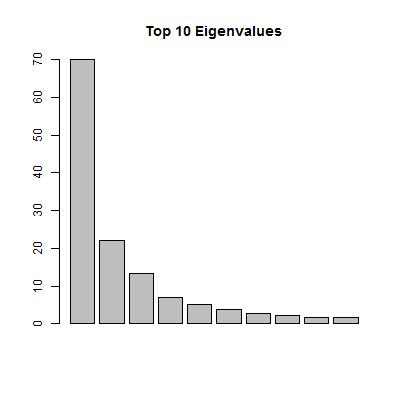
\includegraphics[scale = 0.8]{barplot.jpeg} \\
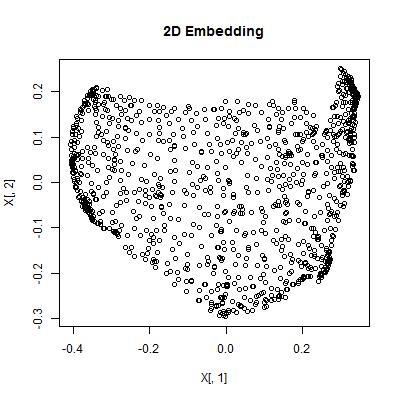
\includegraphics[scale = 0.8]{embedding.jpeg} \\
\end{document}